\documentclass[conference]{IEEEtran}

\usepackage[colorlinks=true, linkcolor=blue, urlcolor=blue, citecolor=blue]{hyperref}
%\usepackage{natbib}
\usepackage{cite}
\usepackage{amsmath,amssymb,amsfonts}
\usepackage{algorithmic}
\usepackage{graphicx}
\usepackage{textcomp}
\usepackage{xcolor}
\usepackage{url}
\usepackage{float}
\usepackage{subcaption}
\usepackage{listings}

\def\BibTeX{{\rm B\kern-.05em{\sc i\kern-.025em b}\kern-.08em
    T\kern-.1667em\lower.7ex\hbox{E}\kern-.125emX}}
%\usepackage[T1]{fontenc}%

%\usepackage[no-math]{fontspec}
%   \setmainfont{Linux Libertine O}
%   \setsansfont{Linux Biolinum O}
%\usepackage{unicode-math}
%   \setmathfont{Asana Math}
\pagenumbering{arabic}

\pagestyle{plain}

\begin{document}
\title{Parallelization of classical molecular dynamics with OpenMP
\\
}
\author{\IEEEauthorblockN{Samuel Moerman}
\IEEEauthorblockA{\textit{Dept.\ of Computer Science} \\
\textit{New York University}\\
New York, USA \\
shm9853@nyu.edu}
\and
\IEEEauthorblockN{Anway Agte}
\IEEEauthorblockA{\textit{Dept.\ of Computer Science} \\
\textit{New York University}\\
New York, USA \\
ama10345@nyu.edu}
\and
\IEEEauthorblockN{Atmaj Koppikar}
\IEEEauthorblockA{\textit{Dept.\ of Computer Science} \\
\textit{New York University}\\
New York, USA \\
ark9238@nyu.edu}
\and
\IEEEauthorblockN{Mihir Prajapati}
\IEEEauthorblockA{\textit{Dept.\ of Computer Science} \\
\textit{New York University}\\
New York, USA \\
jo1449@nyu.edu}
}

\maketitle
\thispagestyle{plain}


\begin{abstract}
We will parallelize a molecular dynamics simulation
\end{abstract}

\begin{IEEEkeywords}
OpenMP, Molecular Dynamics
\end{IEEEkeywords}

\section{Introduction}
Molecular dynamics is a technique to gain insight into the properties of molecules, compounds and materials by
simulating the behavior on a molecular scale. 


Molecular dynamics is based on the integration of Newton's equations of motion. For a system of N particles, this
 corresponds to the following equation:
\begin{align}
    m_i \frac{d^2\mathbf{r}_i}{dt^2} = \mathbf{f}_i = -\frac{\delta}{\delta \mathbf{r}_i}V(\mathbf{r}_1,\mathbf{r}_2,\ldots,\mathbf{r}_N)
\end{align}
Where $\mathbf{r}_1,\mathbf{r}_2,\ldots,\mathbf{r}_N$ represent the set of nuclear coordinates of the N-particle system, 
$V(\mathbf{r}_1,\mathbf{r}_2,\ldots,\mathbf{r}_N)$ the potential energy in function of these coordinates, $\mathbf{f}_i$
the force acting on particle $i$ and $m_i$ the mass of particle $i$. This forms a system of non-linear differential 
equations, which is not solvable analytically. The simulations use a numerical integration algorithm to iteratively
calculate the positions and speeds of the particles throughout time. Some commonly used integration algorithms
include Verlet integration or Langevin integration. More details on the numerical integration can be found in 
% the reference work of Daan Frenkel and Berend Smit. \cite{frenkel2001understanding} 
% \cite{barducci2011metadynamics} \cite{sutto2012new} \cite{bussi2020using}


In order to accomplish this, two components are needed. First a
molecular dynamics engine is required, that is able to calculate the forces on the particles in the system and
integrate these forces through time. The second thing is a force field, which is a set of parameters that are
used by the molecular engine to ensure that the predicted behavior corresponds to the experimental behavior in reality.

In this paper, we set out to write and parallelize a molecular dynamics engine, which is able to simulate some of the
fores of the system.

\begin{figure}[H]
    \centering
    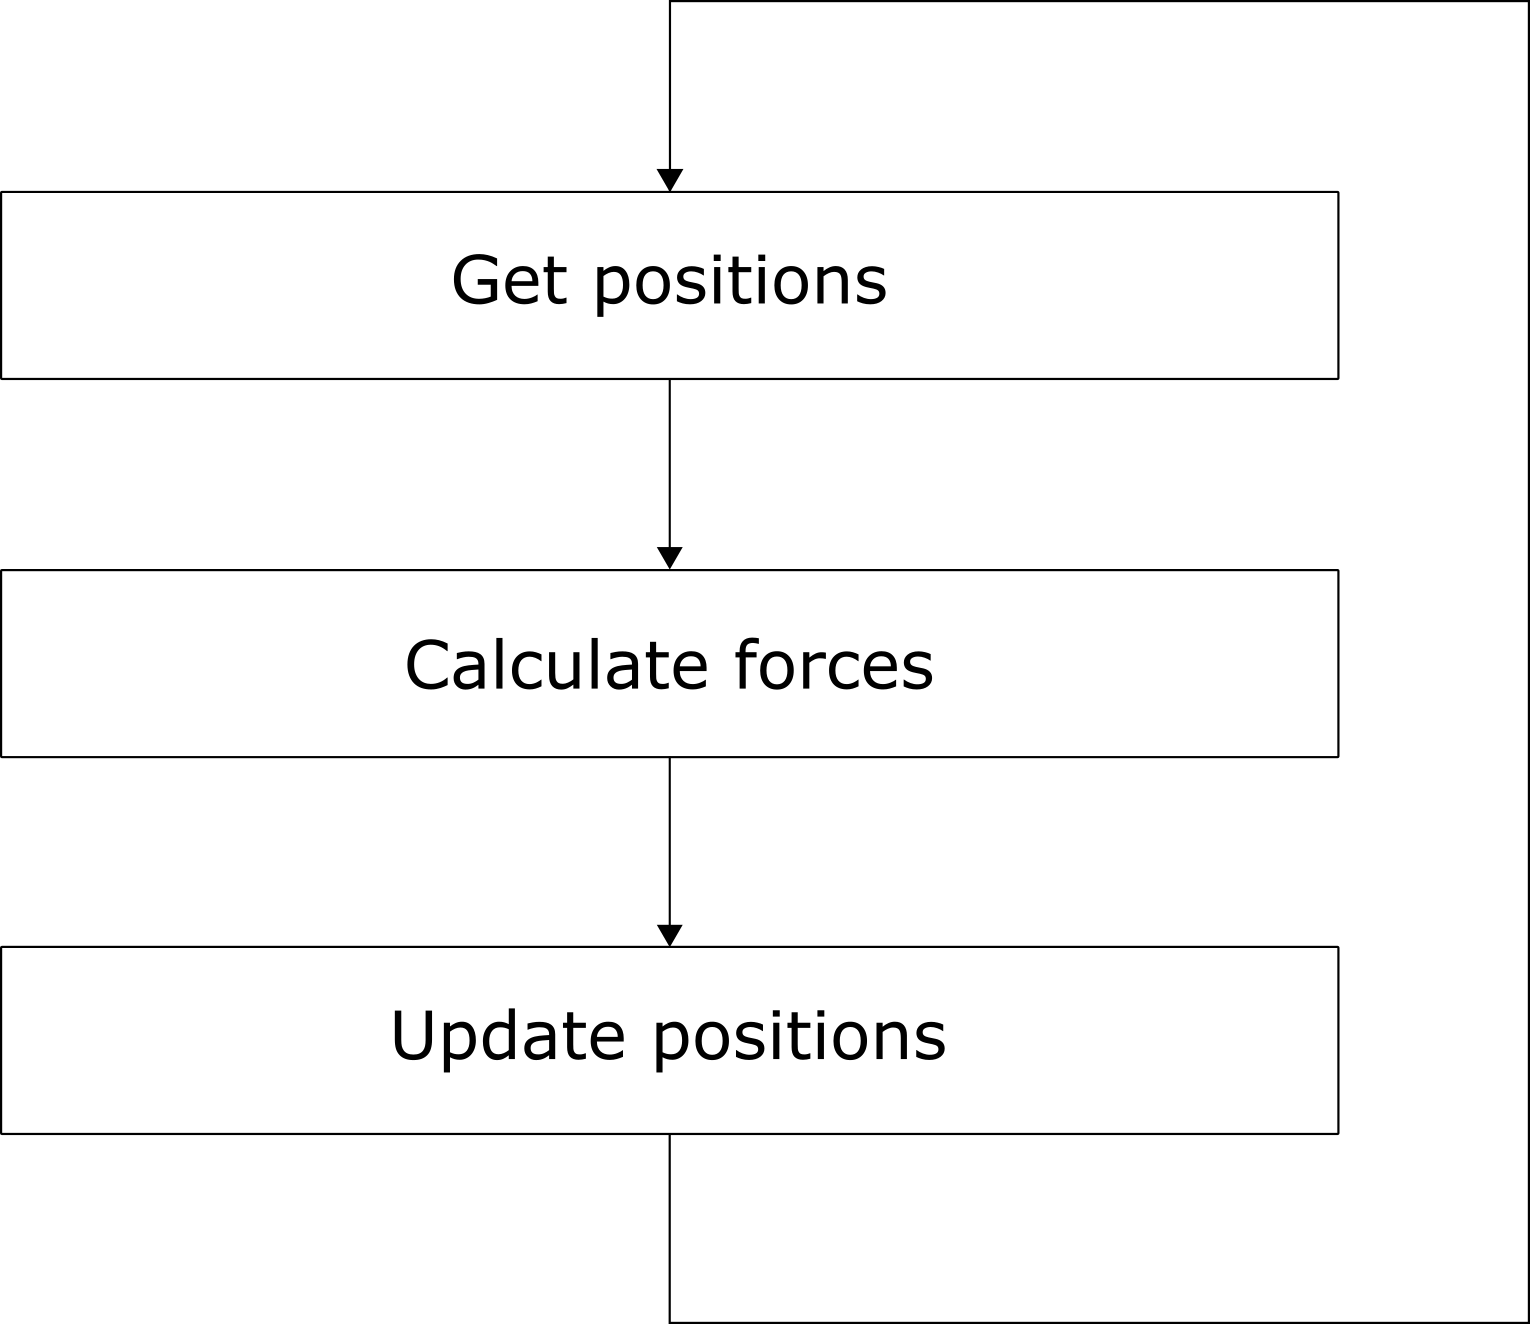
\includegraphics[width=0.7\linewidth]{images/verlet_concept.png}
    \caption{Conceptual visualization of the core concept behind molecular dynamics}
\end{figure}

I LOVE OPENMM.\cite{eastman2010openmm}



\section{Molecular Dynamics Engine}

Organic molecules and biological macromolecules are typically described with the following expression:
\begin{equation}
    \begin{aligned}
    V(\mathbf{r}_1,\mathbf{r}_2,\ldots,\mathbf{r}_N) &= V_{\mathrm{bonds}} + V_{\mathrm{angles}} + 
                                                        V_{\mathrm{dihedrals}}\\
                                                    &+ V_{\mathrm{impropers}} + V_{\mathrm{dispersion \: interaction}}\\
                                                    &+ V_{\mathrm{electrostatic \: interaction}}
    \end{aligned}
\end{equation}
where $\mathbf{r}_1,\mathbf{r}_2,\ldots,\mathbf{r}_N$ are the particles in the system, $V$ is the potential energy of the
system in function of these particles, $V_{\mathrm{bonds}}$ the potential related to the bonds, $V_{\mathrm{angles}}$ 
the potential related to the angles, $V_{\mathrm{dihedrals}}$ the potential related to the dihedrals, 
$V_{\mathrm{impropers}}$ the potential related to the improper torsions, $V_{\mathrm{dispersion \: interaction}}$ 
the potential related to the dispersion interaction and $V_{\mathrm{electrostatic \: interaction}}$ the potential 
related to the electrostatic interaction. 

As described above, the formula consists of different types of potentials.
The term $V_{\mathrm{bonds}}$ can be described as follows:
\begin{equation}
    \begin{aligned}
    V_{\mathrm{bonds}} &= \sum_{\mathrm{bonds}} \frac{k_d}{2}*{(d-d_0)}^2
    \end{aligned}
\end{equation}
where $d$ is the distance between two particles, $d_0$ the standard bond distance for that particular combination of 
particles and $k_d$ the parameter associated with that specific bond. Not that this term is a sum of harmonic 
potentials. The energy increases as the bond distance deviates from the standard bond distance. When the bond 
distance reaches the standard bond distance, the energy associated with this bond becomes zero, which corresponds 
to a harmonic oscillator in a vacuum. The $k_d$ variable is part of the set of parameters specific to the 
forcefield as discussed above.

The term $V_{\mathrm{angles}}$ can be described in a similar way:
\begin{equation}
    \begin{aligned}
    V_{\mathrm{angles}} &= \sum_{\mathrm{angles}} \frac{k_{\theta}}{2}{(\theta-\theta_0)}^2
    \end{aligned}
\end{equation}
where $\theta$ represents the angle between a given set of 3 particles, $\theta_{0}$ the standard angle for this 
particular set and $k_{\theta}$ the parameter associated with that specific angle. The interpretation of this 
term is similar to $V_{\mathrm{bonds}}$, in that a deviation from the standard angle results in an increased energy.

A final term which is described by means of a harmonic oscillator is the term $V_{\mathrm{impropers}}$, which is 
often introduced to  maintain planarity of groups with a flat geometry or sometimes to preserve chirality:
\begin{equation}
    \begin{aligned}
    V_{\mathrm{impropers}} &= \sum_{\mathrm{impropers}} \frac{k_{\psi}}{2}{(\psi-\psi_0)}^2
    \end{aligned}
\end{equation}
where $\psi$ represents the angle between a set of 3 particles, $\psi_0$ the standard improper angle for that 
particular combination of particles and $k_{\psi}$ the parameter associated with that specific improper angle. 
Again, the interpretation is similar to $V_{\mathrm{bonds}}$, in that a deviation from the standard dihedral 
angle results in an increased energy.

The dihedral terms, also referred to as torsion terms, are responsible for introducing an energy barrier to the 
rotation of bonds which do not rotate freely. They can be expressed as follows:
\begin{equation}
    \begin{aligned}
    V_{\mathrm{dihedrals}} &= \sum_{\mathrm{dihedrals}} \frac{k_{\phi}}{2}(1+\cos(n\phi-\phi_0))
    \end{aligned}
\end{equation}
where $\phi$ represents the dihedral angle between a set of 4 particles, $\phi_0$ the standard dihedral angle for 
that particular set of particles, $k_{\phi}$ the parameter associated with that particular dihedral angle and $n$ 
the amount of minima in the rotational profile. The torsion terms are periodic in function of $\phi$ and are 
defined by two additional parameters, $n$ and $\phi_0$. Parameter $n$ refers to the number of minima in the 
rotational profile and is also known as the multiplicity of the function. The parameter $\phi_0$ is known as 
the phase factor, which determines the location of the minima. Often, the rotational profile of a dihedral 
function is not represented by one torsion function, but by a sum of multiple functions. 

The dispersion interaction $V_{\mathrm{dispersion \; interaction}}$ or van der Waals interaction is represented by 
the Lennard-Jones 12\-6 potential and can be rewritten as follows:
\begin{equation}
    \begin{aligned}
    V_{\mathrm{dispersion \; interaction}} &= \sum_{\mathrm{\substack{\mathrm{non-bonded} \\ \mathrm{pairs(i,j)}}}} 4\varepsilon_{ij}\left[
    {\left(\frac{\sigma_{ij}}{r_{ij}}\right)}^{12} - {\left(\frac{\sigma_{ij}}{r_{ij}}\right)}^6
    \right]
    \end{aligned}
\end{equation}
where $r_{ij}$ is the distance between a set of particles $(i,j)$, $\varepsilon_{ij}$ the maximum depth of the 
potential well for this set and $\sigma_{ij}$ the distance between this set where the interaction is zero. This 
interaction takes into account both the attractive and the repulsive aspect of non-bonded interaction. 

The electrostatic interaction $V_{\mathrm{electrostatic \; interaction}}$ is represented by Coulomb's law and can 
be rewritten as follows: 
\begin{equation}
    \begin{aligned}
    V_{\mathrm{electrostatic \; interaction}} &= \sum_{\mathrm{\substack{\mathrm{non-bonded} \\ \mathrm{pairs(i,j)}}}} \frac{q_i q_j}{4\pi\varepsilon_0r_{ij}}
    \end{aligned}
\end{equation}
where $r_{ij}$ is the distance between a set of particles $(i,j)$, $q_i$ and $q_j$ are the charges on particles $i$ 
and $j$ respectively and $\varepsilon_0$ the electric constant. In reality, charges are dispersed throughout a 
molecule. Many forcefields, however, calculate electrostatic interaction by using Coulomb's law, assuming all charges 
are static and can be represented as point charges. 

The Verlet integrator is a commonly used algorithm in molecular dynamics simulations to integrate Newton's equations 
of motion. It is favored for its numerical stability and time-reversibility properties. The positions of particles 
at time \( t + \Delta t \) are calculated based on their positions at time \( t \) and \( t - \Delta t \), along 
with the forces acting on them. The formula is given as follows:
\begin{align}
    \mathbf{r}_i(t + \Delta t) &= 2\mathbf{r}_i(t) - \mathbf{r}_i(t - \Delta t) + \Delta t^2 \cdot \frac{\mathbf{F}(t)}{m},
\end{align}

where \( \mathbf{r}(t) \) is the position of the particle at time \( t \), \( \Delta t \) is the integration time 
step, \( \mathbf{F}(t) \) is the force acting on the particle at time \( t \), and \( m \) is the particle's mass.

This method explicitly depends on the current and previous positions of the particle, eliminating the need to directly 
compute velocities. However, velocities can still be calculated as a midpoint approximation:

\begin{equation}
    \begin{aligned}
    \mathbf{v}(t) &= \frac{\mathbf{r}(t + \Delta t) - \mathbf{r}(t - \Delta t)}{2\Delta t}.
    \end{aligned}
\end{equation}

% The Verlet integrator is particularly suitable for simulations of molecular systems where forces derive from complex potential energy terms, such as:

% \begin{itemize}
%     \item Bond stretching and angle bending potentials (e.g., \( V_{\mathrm{bonds}}, V_{\mathrm{angles}} \)).
%     \item Dihedral and improper torsional potentials (e.g., \( V_{\mathrm{dihedrals}}, V_{\mathrm{impropers}} \)).
%     \item Non-bonded interactions like Lennard-Jones and Coulombic potentials (e.g., \( V_{\mathrm{dispersion}}, V_{\mathrm{electrostatic}} \)).
% \end{itemize}

Because the Verlet algorithm calculates positions and approximates velocities at a single time step, it allows for 
efficient computation without sacrificing accuracy in simulations of large molecular systems.


\section{Literature Review}
    Molecular dynamics is a concept that is inherently very suited to parallelization. Because the forces that
    drive the behavior of the system are comprised of the sum of interactions between sets of particles, a parallelization
    can be performed over these interactions. Moreover, because the technique is inherently an approximative technique,
    there is lots of freedom to further optimize the calculations by using smart approximative algorithms. 

    In general, there are two main approaches that can be taken to improve the performance of the
    simulation engine. Spatial decomposition techniques split the simulation space up and improve performance by
    processing these subregions in parallel. Force decomposition techniques are approximations based on physical grounds
    that improve performance by reducing number of interaction pairs that need to be studies.

    \subsection{Spatial Decomposition Methods}

        \subsubsection{Domain Decomposition}
        Spatial decomposition methods are a fundamental approach to parallelizing MD simulations. The central idea is to 
        split the simulation region into boxes that are then independently processed. The volume of
        these boxes is chosen such that the load between the cores is optimally balanced. More modern approaches often
        tackle this issue in a dynamic fashion, by readjusting the boxes as the simulation progresses.


        Each of the processors is responsible for simulating the behavior of the particles in that region. One of the main
        challenges of this approach is how the interfaces between the subdivisions are handled. 

        \subsubsection{Neighbor Lists}
        Neighbor list is another spatial decomposition approach that can be used to parallelize MD simulations. The
        core idea is to maintain a list of potential interaction partners for each particle in the system. This
        significantly reduces the time complexity, given that the algorithm no longer needs to iterate over all
        atom pairs ($O(N)$), but only needs to iterate over the neighbor list for each particle ($O(N)$). These
        techniques are especially relevant for short-range non-bonded interactions.



    \subsection{Force Decomposition Methods}
    % Because classical molecular dynamics are based on Newton's third law of motion, a skew-symmetric
    % force matrix $f$ can be defined as follows
    % \begin{align*}
    %         f =
    %         \begin{bmatrix}
    %         0 & f_{12} & f_{13} & \cdots & f_{1N} \\
    %         -f_{12} & 0 & f_{23} & \cdots & f_{2N} \\
    %         -f_{13} & -f_{23} & 0 & \cdots & f_{3N} \\
    %         \vdots & \vdots & \vdots & \ddots & \vdots \\
    %         -f_{1N} & -f_{2N} & -f_{3N} & \cdots & 0
    %         \end{bmatrix}  
    % \end{align*}
    % of which only the upper or lower triangular portion needs to be calculated.
    % This allows for decomposition based on the interactions between particle pairs. 
    PME methods, .... not sure if this falls under the category of parallelization strategies, more like
    algorithmic strategies I guess

    \subsubsection{Bonded Interactions}
        \subsection{Particle Decomposition Methods}
        \subsubsection{Atom Decomposition}
        This approach generally uses systolic topology for interprocessor communication when replicated data is not 
        possible in each processor

\subsection{Hybrid Parallelization Approaches}

\section{Parallelization}

\subsection{Electrostatic Forces}
In general, the non-bonded interactions (i.e.\ the electrostatic interaction and the dispersion interaction) usually
take up the majority of the time for classical molecular dynamics simulations. This is because these interactions are
two-particle interactions, which would naively require a double loop over all particles resulting in an $O(N^2)$
time complexity. 
\begin{lstlisting}
    compute(system):
        for particles in system:
            for particles in system:
                - calculate distance
                - compute electrostatic force
    \end{lstlisting}


However, because of Newton's third law of motion, we can leverage the concept of a skew-symmetric 
force matrix $f$
\begin{align*}
        f =
        \begin{bmatrix}
        0 & f_{12} & f_{13} & \cdots & f_{1N} \\
        -f_{12} & 0 & f_{23} & \cdots & f_{2N} \\
        -f_{13} & -f_{23} & 0 & \cdots & f_{3N} \\
        \vdots & \vdots & \vdots & \ddots & \vdots \\
        -f_{1N} & -f_{2N} & -f_{3N} & \cdots & 0
        \end{bmatrix}  
\end{align*}
of which only the upper or lower triangular portion needs to be calculated.
\begin{lstlisting}
compute(system):
    for particle pairs in system:
            - calculate distance
            - compute electrostatic force
\end{lstlisting}

This loop is parallelized using a
\verb|collapse(2)| clause, which can since deal with non-rectangular loops since OpenMP 5.1. Additionally, local 
force arrays are created during the force 
\begin{lstlisting}
compute(system):
    #pragma omp for collapse(2)
    for particle pairs in system:
            - calculate distance
            - compute electrostatic force
            - store in local force array

    #pragma omp critical
    - merge local force arrays
    \end{lstlisting}
\section{Results}
In this section, the results of the parallelization strategies will be reported. In order to gain deeper insight into
the performance of the program, a benchmark was performed on different levels of detail. This allows for a more
comprehensive discussion about potential bottlenecks and areas for future work. More specifically, traditional
metrics such as speedup and efficiency were employed to analyze the overall performance of the program. Besides this,
more fine-grained benchmarking was done to gain more insight into how each of the force types performed on an
individual level.

    \subsection{Force Type Parallelization}
    In the following subsections, we will analyze the performance of the program per force type calculation. By
    individually studying each of the implemented force types, a deeper understanding can be gained. A range of 
    systems of different size will be studied.


        \subsubsection{Electrostatic Interaction}
        In Fig. \ref{fig:electro-speedup}, the speedup for a range of different systems is displayed. We can clearly
        see a ... for small systems and ..... for larger systems
        \begin{figure}[H]
            \centering
            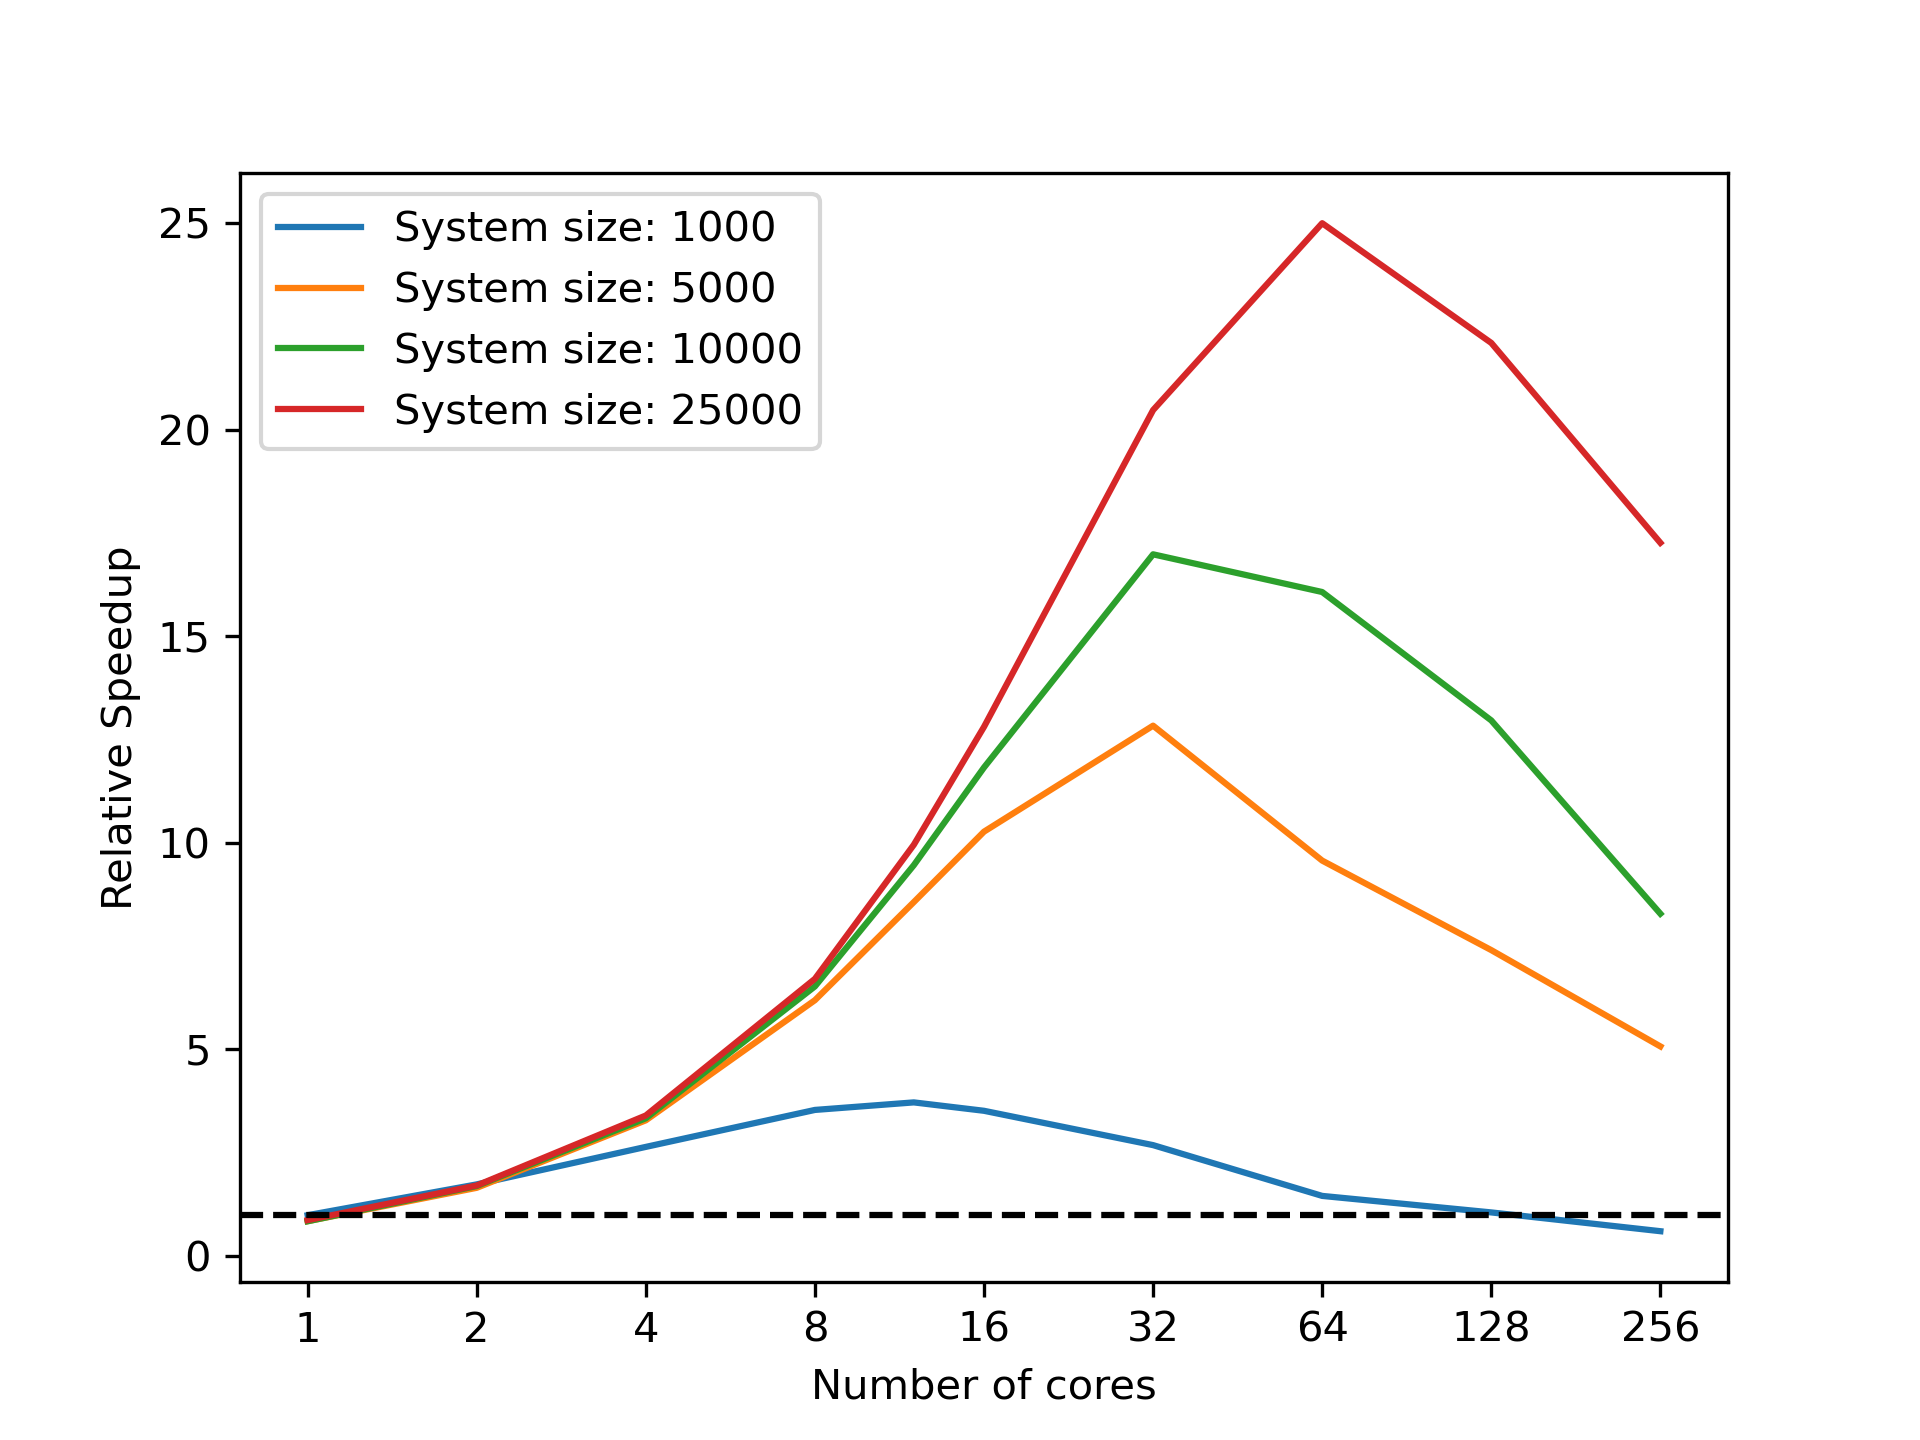
\includegraphics[width=\linewidth]{./images/electrostatic_scaling.png} % This creates a placeholder box with text
            \caption{Speedup of a range of systems containing only electrostatic interaction in function of the number 
            of threads.}\label{fig:electro-speedup}
        \end{figure}


        \subsubsection{Dispersion Interaction}
        In Fig. \ref{fig:dispersion-speedup}, the speedup for a range of different systems is displayed. We can clearly
        see a ... for small systems and ..... for larger systems
        \begin{figure}[H]
            \centering
            \fbox{\textbf{[Image Placeholder]}} % This creates a placeholder box with text
            \caption{Speedup of a range of systems containing only dispersion interaction in function of the number 
            of threads.}\label{fig:dispersion-speedup}
        \end{figure}

        \subsubsection{Bonded Interaction}
        In Fig. \ref{fig:bonded-speedup}, the speedup for a range of different systems is displayed. We can clearly
        see a ... for small systems and ..... for larger systems
        \begin{figure}[H]
            \centering
            \fbox{\textbf{[Image Placeholder]}} % This creates a placeholder box with text
            \caption{Speedup of a range of systems containing only bonded interaction in function of the number 
            of threads.}\label{fig:bonded-speedup}
        \end{figure}
    
    \subsection{Nested Parallelization}
    In this subsection, the nested parallelism over the different force types will be studied. To be honest this will
    be a bit more complicated to write about, or too simple to write much about, not sure yet. Let's discuss this
    after we get the results

\section{Discussion}



\bibliographystyle{plain}
\bibliography{references}

\end{document}
